\chapter{Implementación}

La implementación del software se ha dividido en hitos. Estos han sido definidos en Github
y cada uno de ellos contiene un grupo de \textit{issues} que se corresponden con las distintas
mejoras que se han ido incorporando al software a lo largo de su desarrollo.\\

\section{Primer hito: Creación de la infraestructura del proyecto}

Este fue el primer hito abordado dentro del proyecto. Se trata de un hito interno cuya función es crear el esqueleto del proyecto.
Su objetivo, una vez estructurado el proyecto es obtener un módulo compilable que defina la estructura de datos.

Para completar este hito, se han tenido que tomar una serie de decisiones respecto a los temas que se exponen a continuación.
\newpage

\subsection{Elección de un Bot para comunicar los cambios por telegram \cite{telegram}}

\subsubsection{Criterios}
Para la elección del bot que comunique en telegram los cambios
efectuados en este repositorio tendremos en cuenta los siguientes
criterios:

\begin{itemize}
    \item Debe ser un bot gratuito
    \item Posibilidad de notificar tanto
de push como de creación de pull requests e issues
    \item La puesta a punto
y configuración sea la menor posible.
    \item Se pueda contestar a los issues
directamente desde Telegram.
\end{itemize}

\subsubsection{Opciones}
Las 2 opciones que se han contemplado han sido las siguientes:\\

\textbf{Crear un bot de telegram y hacer que este notifique los
cambios usando GitHub
Actions:}
\begin{itemize}
    \item Es gratuito
    \item Puede notificar de todas las acciones
    \item Se necesita configurar desde 0
    \item No se pueden contestar a los issues desde Telegram
\end{itemize}

\textbf{GitHubBot:}
\begin{itemize}
    \item Es gratuito
    \item Puede notificar de todas las acciones indicadas
    \item Ya viene configurado y su puesta a punto es sencilla.
    \item Se pueden contestar a los issues desde Telegram
\end{itemize}

\subsubsection{Elección}

Debido a la facilidad de tenerlo configurado para todos los tipos de
eventos y junto a la posibilidad de responder directamente desde
Telegram he decidido usar GitHubBot como bot que notifique los cambios del
repositorio.\\

\subsection{Elección del lenguaje a usar}

En este punto del proyecto, llegó el momento de elegir qué lenguaje iba a usar. Para este proyecto, tenía intención de usar un
lenguaje que no hubiera usado anteriormente, para aprovechar la oportunidad de conocer un nuevo lenguaje.\\

Finalmente, decidí optar por Go, ya que aparte de ser uno de los lenguajes que tenía intención de aprender en un futuro, tiene ciertas
características que me terminaron por convencer. Entre ellas destacan las siguientes:

\begin{itemize}
    \item Código abierto
    \item Es un lenguaje muy rápido en comparación con el resto de lenguajes compilados
    \item Es un lenguaje orientado a objetos 
    \item Soporta miles de conexiones en el mismo programa
\end{itemize}

\newpage

\subsection{Gestor de dependencias}
\subsubsection{Criterios}

\begin{itemize}
\item
  Mejores prácticas del lenguaje (GO)
\item
  Freshness
\item
  Comunidad activa
\end{itemize}

\subsubsection{Posibles opciones y elección}

En el caso de los proyectos en GO, los diferentes criterios para elegir
un gestor de dependencias llevan siempre a la misma opción:
Go Modules \cite{go-modules}, el propio
gestor de dependencias de Go, lanzado en 2019 y que solucionaba la
problemática que tenían los proyectos en Go con la gestión de
dependencias.

El único gestor de dependencias que podría intentar ser una opción
frente a Go Modules es Dep \cite{dep}, gestor
de dependencias que se usaba antes de la existencia de Go Modules, pero
que dejaron de mantener cuando este salió a la luz y actualmente está
deprecado.

Por lo tanto, en este proyecto se ha elegido usar Go Modules como gestor
de dependencias.

\newpage
\subsection{Gestor de tareas}
\subsubsection{Criterios}\label{criterios}

\begin{itemize}
\item
  Freshness
\item
  Facilidad para entender la sintaxis y poder crear y ampliar las tareas
\item
  Facilidad para instalar el gestor y empezar a usarlo
\end{itemize}

\subsubsection{Posibles opciones}
Tras hacer una búsqueda de las posibles opciones se han llegado a 2
posibles candidatos a ser el gestor de tareas del proyecto: Make y Task.
A continuación, se describirán con más detalle ambos gestores en función
de los criterios de elección para llegar a la conclusión de cuál de las
2 opciones es la más adecuada para este proyecto.\\

\textbf{Make \cite{make}}

\begin{itemize}
\item
  Gestor de tareas más popular, lo que conlleva una comunidad más amplia
  y activa, por lo tanto, una mayor facilidad para encontrar la solución
  a posibles problemas.
\item
  El abanico de posibilidades que ofrece esta herramienta es más amplio
  que la competencia, debido a que es una herramienta más antigua y
  asentada.
\item
  No está creada originalmente para trabajar con lenguajes como Go, pero
  se adapta y es una herramienta perfectamente usable.
\item
  Considero que la sintaxis es más complicada y menos legible que la
  competencia.
\item
  En cuanto a freshness, es un gestor que lleva actualizandose
  frecuentemente desde antes de los 80 y su última actualización fue a
  finales de 2022. Cosas como esta hacen que aunque pasen los años siga
  siendo el gestor de tareas más popular.
\item
  Su instalación no es complicada
\end{itemize}

\textbf{Task \cite{task}}

\begin{itemize}
\item
  Gestor de tareas bastante popular, con una comunidad activa y escrito
  y pensado para usarse en proyectos de Go.
\item
  Su abanico de posibilidades no es tan amplio como el de Make, pero esa
  diferencia no tiene ninguna repercusión en el ámbito que afecta a este
  proyecto.
\item
  Su sintaxis es mucho más sencilla y el
  \href{https://taskfile.dev/usage/}{`Get started'} es bastante sencillo
  e intuitivo.
\item
  En cuanto a freshness, al ser una herramienta menos amplia que make,
  necesita menos actualizaciones, ya que lo único que han hecho ha sido
  ir sacando pequeñas mejoras. Sin embargo, podemos ver en su
  \href{https://github.com/go-task/task}{página de GitHub} que siguen
  habiendo aportaciones recientes. Esto nos hace ver que la herramienta
  sigue estando a la orden del día por lo que cumple el criterio de
  frescura aunque considero que no llega a tener la frescura que puede
  tener make debido a que es una herramienta mucho más grande. Pero para
  este proyecto, no considero que esta diferencia pueda generar problema
  alguno.
\item
  Su instalación no es complicada.
\end{itemize}


\textbf{Elección}

\begin{itemize}
\item
  Debido a facilidad de uso y complejidad de sintaxis, he elegido que
  Task será el gestor de tareas elegido para este proyecto. Esta
  elección viene dada porque considero que los pros (facilidad de uso y
  complejidad de sintaxis más sencilla) son más relevantes para este
  proyecto que los contras (abanico de posibilidades del gestor y
  freshness)
\end{itemize}

\textbf{Instalación de Task}

La misma página oficial te da un abanico de posibilidades para
\href{https://taskfile.dev/installation/}{instalar Task}

\newpage
\section{Segundo hito: Implementación de la lógica de negocio necesaria para la creación de 2 equipos igualados}

En este hito se pretende implementar la lógica de negocio necesaria para poder crear 2 equipos igualados en función del nivel de todos los participantes.
Para darlo por concluido, se debe poder añadir jugadores al grupo, cambiar su disponibilidad y crear equipos igualados entre los jugadores disponibles.
Los tests relacionados con las funcionalidades mencionadas deben lanzarse automáticamente.

Para conseguir completar este hito, se han tenido que tomar una serie de decisiones en función de los siguientes temas:

\subsection{Biblioteca aserciones}

\subsubsection{Criterios}

\begin{itemize}
\item
  Mejores prácticas para Go (Bibliotecas referenciadas como paquetes
  disponibles por la página oficial de Go \cite{go-dev}).
\item
  Biblioteca que permita testear los errores.
\item
  Freshness.
\item
  Valoración en Go Report Card \cite{go-report-card}.
\end{itemize}

\subsubsection{Opciones}

\textbf{Biblioteca estándar de testing para
Go}

\begin{itemize}
\item
  \href{https://pkg.go.dev/testing}{Aquí} \cite{go-dev} podemos ver la documentación
  acerca de la forma de testear nativa de Go, la cual no incluye
  funciones de aserción y se deben comparar los resultados manualmente.
\item
  Al hacer las aserciones mediante comparaciones, si permite el testeo
  de errores.
\item
  Al ser el paquete de testing oficial del lenguaje, cumple el requisito
  de freshness.
\item
  De la misma manera, al ser un paquete propio de Go, no tiene reporte
  en Go Report Card.
\end{itemize}

\textbf{BE}

\begin{itemize}
\item
  \href{https://pkg.go.dev/github.com/carlmjohnson/be}{Aquí} se puede
  ver la documentación sobre BE en la página de Go.
\item
  Al ser un paquete muy minimalista, no es una biblioteca apta para el
  testeo de errores.
\item
  Cumple el criterio de frescura, ya que es una biblioteca nueva, estable
  y en continua actualización.
\item
  Tiene una puntuación de
  \href{https://goreportcard.com/report/github.com/carlmjohnson/be}{A+}
  en Go Report Card.
\end{itemize}

\textbf{Testify}

\begin{itemize}
\item
  \href{https://pkg.go.dev/github.com/stretchr/testify}{Aquí} \cite{go-dev} se puede
  ver la documentación sobre Testify en la página de Go.
\item
  Debido a su alto abanico de funciones tiene una gran parte de estas
  dedicada al testeo de errores.
\item
  Es una herramienta activa y en continua actualización.
\item
  Tiene una puntuación de
  \href{https://goreportcard.com/report/github.com/stretchr/testify}{A+}
  en Go Report Card.
\end{itemize}

\textbf{Assert}

\begin{itemize}
\item
  \href{https://pkg.go.dev/gopkg.in/go-playground/assert.v1}{Aquí} se
  puede ver la documentación sobre Assert en la página de Go.
\item
  El hecho de ser un paquete básico tiene el problema de no tener un
  amplio abanico de funciones y esto repercute en la limitación de poder
  testear los errores.
\item
  Es una herramienta activa y estable.
\item
  Tiene una puntuación de
  \href{https://goreportcard.com/report/github.com/go-playground/assert}{A+}
  en Go Report Card.
\end{itemize}

\textbf{Gomega}

\begin{itemize}
\item
  \href{https://pkg.go.dev/github.com/onsi/gomega}{Aquí} \cite{go-dev} se puede ver la
  documentación sobre Gomega en la página de Go. Aquí podemos ver que
  este framework está orientado a BDD, y no a TDD como el resto de
  opciones que se han contemplado.
\item
  Al tener otro enfoque de testeo, y en este caso se busca testear el
  comportamiento de un usuario promedio y no entrar en implementación,
  no está enfocado para testear errores.
\item
  Es una biblioteca actualizada y activa.
\item
  Tiene una puntuación de
  \href{https://goreportcard.com/report/github.com/onsi/gomega}{A+} en
  Go Report Card.
\end{itemize}

\subsubsection{Elección}

Debido a que es la opción más completa, tiene una buena cantidad de
funciones enfocada al testeo de errores y está enfocada en TDD, se
optará por usar Testify como biblioteca de aserciones. Se puede acceder a
la guía de instalación
\href{https://pkg.go.dev/github.com/stretchr/testify\#section-readme}{en
el siguiente enlace} \cite{go-dev}.

\subsection{Test runner}

\subsubsection{Criterios}

\begin{itemize}
\item
  Mejores prácticas para Go
\item
  Facilidad para lanzar y gestionar los tests
\end{itemize}

\subsubsection{Elección}

La elección del test runner en este caso es sencilla, ya que el propio Go
tiene un test runner propio, el cual hace que sea muy sencillo lanzar y
gestionar los tests. Además, no se ha encontrado ninguna alternativa
real que ofrezca algún motivo por el que utilizarla en vez del test runner
nativo de Go.

\subsection{Elección de la imagen base del contenedor que se usará para lanzar los tests}

\subsubsection{Criterios}

Para la elección de la imagen base se seguirán las mejores prácticas, lo
que consiste en:

\begin{itemize}
\item
  Priorizar la imagen de menor peso posible que satisfaga nuestras
  necesidades. (Evitar imágenes que incluyan paquetes o funcionalidades
  que no se vayan a usar para el testing)
\item
  Freshness
\end{itemize}

\subsubsection{Opciones}

Tras ver las \href{https://hub.docker.com/_/golang}{imágenes oficiales} \cite{dockerhub}
que nos proporciona DockerHub con la versión de Go 1.20 y tras descartar
ciertas como WindowsServer y NanoServer debido a que están basadas en
windows tenemos las siguientes opciones, las cuales cumplen el criterio
de frescura, ya que son imágenes oficiales y siempre están en continua
actualización:

\begin{itemize}
\item
  Alpine: Tamaño comprimido = 100 MB , Tamaño de la imagen una vez
  pulleada = 253 MB.
\item
  Buster: Tamaño comprimido = 282 MB , Tamaño de la imagen una vez
  pulleada = 720 MB.
\item
  Bullseye: Tamaño comprimido = 300 MB , Tamaño de la imagen una vez
  pulleada = 777 MB.
\end{itemize}

Pasando a las no oficiales, encontramos las siguientes opciones
(descartando las que apenas tienen descargas o llevan mucho tiempo sin
ser actualizadas):

\begin{itemize}
\item
  \href{https://hub.docker.com/r/circleci/golang}{CircleCi}: Su tamaño
  comprimido es 1GB, por lo que ni se acerca a las imágenes oficiales.
  Su última versión es para Go 1.17, lo que lo hace también estar peor
  posicionado que las oficiales elegidas, ya que no cumple con el
  criterio de frescura al llevar más de un año sin actualizarse.
\item
  \href{https://hub.docker.com/r/okteto/golang}{Okteto}: Su tamaño
  comprimido es de 400MB, que aunque mejora al de CircleCi, está aún por
  encima de las imágenes oficiales. Su última versión es para Go 1.18,
  lo que lo hace también estar peor posicionado que las oficiales
  elegidas. Su última actualización fue hace 15 días, por lo que cumple
  con el criterio de frescura.
\item
  \href{https://hub.docker.com/r/bitnami/golang}{Bitnami (by VMware)}:
  Tamaño comprimido de 289MB y última versión 1.19.5, la misma que las
  imágenes oficiales, lo que hace que se posicione muy bien en cuanto a
  frescura, pero es casi 3 veces más pesada que la mejor opción de las
  imágenes oficiales.
\item
  \href{https://hub.docker.com/r/antrea/golang}{Antrea}: También
  pertenece a VMware, pero la imagen base es aún más pesada que la
  opción anterior y aunque a día de hoy se sigue actualizando, su
  versión actual está por detrás que la de Bitnami y las imágenes
  oficiales.
\item
  \href{https://hub.docker.com/r/corpusops/golang}{CorpusOps}:
  Encontramos una imagen basada en Alpine la cual mejora a algunas de
  las imágenes oficiales en cuanto a peso (171MB), pero es más pesada
  que la imagen de alpine oficial, la cual, pese a ambas estar en
  continua actualización a día de hoy, está por delante en cuanto a
  versión de Go.
\item
  \href{https://hub.docker.com/r/clearlinux/golang}{ClearLinux}: Tamaño
  comprimido de +1GB. Cumple con el criterio de frescura, ya que se
  actualizó hace 1 semana.
\item
  \href{https://hub.docker.com/r/alpinelinux/golang}{AlpineLinux}:
  Opción interesante debido a su poco peso (193 MB), pero es más pesada
  que la imagen oficial de Go sobre Alpine. Cumple con el criterio de
  frescura, ya que su última actualización fue hace 3 días.
\end{itemize}

\subsubsection{Elección}

Debido al tamaño y a que las mejores prácticas sugieren usar esta imagen
base se ha elegido la versión oficial de Go sobre Alpine. Se usará el
tag ``alpine'', el cual apunta siempre a la última versión oficial de Go
sobre Alpine lanzada.

\newpage
\subsection{Elección del Sistema de CI}

\subsubsection{Criterios}

\begin{itemize}
\item
  Sistema que tenga la posibilidad de usar GitHub Checks API (Si para
  esto se necesita instalar una aplicación en GitHub, buscar opciones
  cuyas aplicaciones tengan un número de descargas aceptable para
  aumentar la fiabilidad)
\item
  Que permita usar el sistema de manera gratuita para proyectos públicos
\item
  Sistemas que permitan trabajar con Docker
\end{itemize}

\subsubsection{Opciones}

Se ha descartado Jenkins, ya que aunque es una de las opciones más
populares, no tiene una versión gratuita.

\textbf{GitHub Actions \cite{actions}}

\begin{itemize}
\item
  Al ser propio de GitHub usa Checks API
\item
  Es gratuito para proyectos públicos
\item
  Permite trabajar con Docker
\end{itemize}

\textbf{CircleCi \cite{circle-ci}}

\begin{itemize}
\item
  Usa Checks API
\item
  Es gratuito
\item
  Permite trabajar con Docker
\end{itemize}

\textbf{SemaphoreCi  \cite{semaphore-ci}}

\begin{itemize}
\item
  Usa checks API
\item
  Tiene una versión gratuita pero no se puede instalar a GitHub como
  aplicación gratuitamente
\item
  Permite trabajar con Docker
\end{itemize}

\textbf{CirrusCi \cite{cirrus-ci}}

\begin{itemize}
\item
  Usa checks API (Instalando CirrusCi como aplicación en Github
  gratuitamente)
\item
  Es gratis para repositorios públicos
\item
  Permite trabajar con Docker
\end{itemize}

\textbf{TravisCI \cite{travis-ci}}

\begin{itemize}
\item
  Usa checks API (Instalando Travis como aplicación en Github)
\item
  Se puede obtener una prueba gratis, pero es necesario introducir la
  tarjeta de crédito
\item
  Permite trabajar con Docker
\end{itemize}

\subsubsection{Elección}

Entre las opciones plasmadas, se ha descartado CircleCi para evitar la
opción más básica, TravisCi por el hecho de tener que introducir la
tarjeta de crédito y SemaphoreCi debido a que no he llegado a saber a
ciencia cierta si usa GitHub Checks API y si se puede usar de forma
gratuita.

Debido a esto, se usarán las propias GitHub Actions y CirrusCi como
sistemas de CI.

\subsection{Versiones de Go testeadas}

Se han consultado \href{https://endoflife.date/go}{las versiones de Go
que siguen teniendo soporte} y basándonos en esta información se han
testeado las siguientes versiones:

\begin{itemize}
\item
  1.20: Versión que acaba de salir y que se testea mediante CirrusCi con
  el contenedor del Objetivo 5, que se construye siempre con la última
  versión de Go.
\item
  1.19: Versión que aún tiene soporte y se testea mediante GitHub
  actions.
\item
  1.18: Versión que ha dejado de tener soporte el 1 de Febrero, pero se
  ha testeado también por la brevedad de tiempo que lleva sin ser tener
  soporte. También se testea mediante GitHub actions.
\end{itemize}

\section{\href{https://github.com/manujurado1/SportsBar-IV/tree/PMV-Estructuras_de_datos}{Tercer hito:  Diseñar correctamente todas las estructuras de datos necesarias usando DDD}} 

En este hito se abordó una reestructuración de la estructura de datos creada dos hitos atrás, ya que se identificó que esta no era 
la más oportuna para el proyecto. Debido a eso, no hubo que tomar ninguna decisión extra, ya que las tomadas en el hito 1 si que eran válidas.

\section{\href{https://github.com/manujurado1/SportsBar-IV/tree/PMV-Logica_de_negocio}{Cuarto hito: Implementación de la lógica de negocio}}

En este hito, esta vez ya sobre una estructura correcta, se implementó la lógica de negocio capaz de generar 2 equipos igualados.
También es implementó la lógica capaz de modificar los niveles de los amigos participantes en un partido en función de su resultado.
Al igual que en el hito anterior, en este no hubo que tomar ninguna decisión ya que estas fueron tomadas 2 hitos atrás.

\newpage
\section{\href{https://github.com/manujurado1/SportsBar-IV/tree/PMV-Creacion_API}{Quinto hito: Creación de la API REST}}

En este milestone se plantea la creación de una API REST para trabajar con la lógica de negocio.

\subsection{Conveniencia de usar un framework para crear la API REST}

\subsubsection{Criterios}

Como criterio a la hora de tomar la decisión de usar o no un \textit{framework} se expondrán los pincipales pros y contras de usar un \textit{framework} o decantarse únicamente por la biblioteca estándar

\subsubsection{Opciones y decisión}

Go nos da la posibilidad de crear una API REST sin necesidad de usar ningún \textit{framework}, gracias a su biblioteca estándar \href{https://pkg.go.dev/net/http}{net/http} \cite{go-dev}.
Aún así, la posibilidad de añadir una capa al proyecto usando algún \textit{framework} para crear la API nos puede otorgar ciertas facilidades a la hora de su creación y de manejar las solicitudes y los errores.

Por lo tanto, debido a que gracias a Go Modules no es un problema añadir dependencias al proyecto, y estas no afectan negativamente al rendimiento del mismo, se ha optado por usar
un framework para crear la API REST, respaldado por las funcionalidades que nos proporciona la bibioteca estándar.

\subsection{Elección del framework para la creación de la API REST}

\subsubsection{Criterios}

\begin{itemize}
\item
  Herramienta que proporcione funciones para la validación de solicitudes y manejo de errores
\item
  Puntuación en \href{https://goreportcard.com/}{Go Report Card} \cite{go-report-card}
\end{itemize}

\subsubsection{Opciones}

\textbf{\href{https://pkg.go.dev/github.com/gin-gonic/gin}{Gin} \cite{go-dev}}

\begin{itemize}
\item
  Ofrece funciones para facilitar la validación de solicitudes y manejo de errores mediante un \textit{middleware}.
\item
  Puntuación A+ en Go Report Card (5 \textit{issues} encontrados)
\end{itemize}

\textbf{\href{https://pkg.go.dev/github.com/labstack/echo/v4}{Echo} \cite{go-dev}}

\begin{itemize}
\item
  Incluye un mecanismo de validación y permite añadir middleware para el manejo de errores
\item
Puntuación A+ en Go Report Card (19 \textit{issues} encontrados)
\end{itemize}

\textbf{\href{https://pkg.go.dev/github.com/gofiber/fiber/v2}{Fiber} \cite{go-dev}}

\begin{itemize}
\item
  Incluye el mismo validador que Echo y tiene una función de manejo de errores integrada.
\item
Puntuación A+ en Go Report Card (38 \textit{issues} encontrados)
\end{itemize}

\subsubsection{Elección}

Una vez expuestos los criterios sobre estas opciones, he decidido decantarme por Gin, debido a que tiene tiene mejores porcentajes en Go Report Card debido a que contiene menos problemas que el resto.
Además aporta facilidades en la validación de solicitudes y manejo de errores.

\newpage

\section{\href{https://github.com/manujurado1/SportsBar-IV/tree/PMV-Despliegue_API}{Sexto hito: Despliegue de la API REST}}
En este último hito del proyecto se ha planteado la puesta a punto y despliegue de la API REST. Para ello se han tenido que realizar las siguientes acciones:

\subsection{Documentación de la API REST}
Ya que la API va a estar disponible para el usuario, es necesaria una buena documentación que permita al usuario conocer el funcionamiento de la API.
En este caso, se ha seguido la especificación de OpenAPI a través de Swagger \cite{swagger}, creando la siguiente documentación:

\begin{figure}[H]
	\centering	
	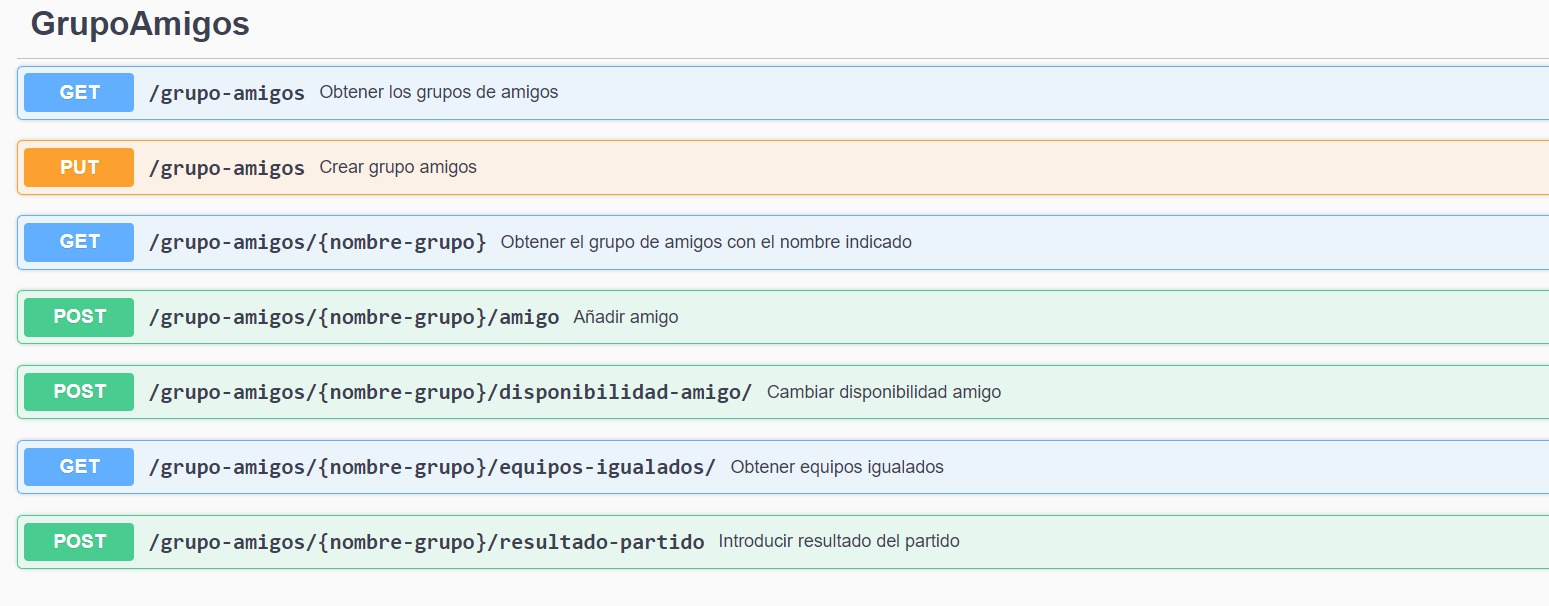
\includegraphics[scale=0.25]{img/doc-api.jpg}
	\caption{Documentación de la API}
\end{figure}

\subsection{Despliegue de la API REST}
Para el despliegue de la API, se ha buscado una aplicación que permitiese desplegar la API de manera gratuita y además, que esta fuera compatible con Go y Gin.
Finalmente se ha elegido hacer el despliegue a través de Render \cite{render}, debido a la facilidad con la que permite desplegar la API, aparte de ser gratuito y soportar proyectos web hechos con Go y Gin.